\iffalse
\let\negthickspace\undefined
\documentclass[journal,12pt,onecolumn]{IEEEtran}
\usepackage{cite}
\usepackage{amsmath,amssymb,amsfonts,amsthm}
\usepackage{algorithmic}
\usepackage{graphicx}
\usepackage{textcomp}
\usepackage{xcolor}
\usepackage{txfonts}
\usepackage{listings}
\usepackage{enumitem}
\usepackage{mathtools}
\usepackage{gensymb}

\usepackage{tkz-euclide} % loads  TikZ and tkz-base
\usepackage{listings}



\newtheorem{theorem}{Theorem}[section]
\newtheorem{problem}{Problem}
\newtheorem{proposition}{Proposition}[section]
\newtheorem{lemma}{Lemma}[section]
\newtheorem{corollary}[theorem]{Corollary}
\newtheorem{example}{Example}[section]
\newtheorem{definition}[problem]{Definition}
%\newtheorem{thm}{Theorem}[section] 
%\newtheorem{defn}[thm]{Definition}
%\newtheorem{algorithm}{Algorithm}[section]
%\newtheorem{cor}{Corollary}
\newcommand{\BEQA}{\begin{eqnarray}}
\newcommand{\EEQA}{\end{eqnarray}}
\newcommand{\system}[1]{\stackrel{#1}{\rightarrow}}

\newcommand{\define}{\stackrel{\triangle}{=}}
\theoremstyle{remark}
\newtheorem{rem}{Remark}
%\bibliographystyle{ieeetr}
\begin{document}
%
\providecommand{\pr}[1]{\ensuremath{\Pr\left(#1\right)}}
\providecommand{\prt}[2]{\ensuremath{p_{#1}^{\left(#2\right)} }}        % own macro for this question
\providecommand{\qfunc}[1]{\ensuremath{Q\left(#1\right)}}
\providecommand{\sbrak}[1]{\ensuremath{{}\left[#1\right]}}
\newcommand{\brac}[1]{\left( #1 \right)}
\providecommand{\lsbrak}[1]{\ensuremath{{}\left[#1\right.}}
\providecommand{\rsbrak}[1]{\ensuremath{{}\left.#1\right]}}
\providecommand{\brak}[1]{\ensuremath{\left(#1\right)}}
\providecommand{\lbrak}[1]{\ensuremath{\left(#1\right.}}
\providecommand{\rbrak}[1]{\ensuremath{\left.#1\right)}}
\providecommand{\cbrak}[1]{\ensuremath{\left\{#1\right\}}}
\providecommand{\lcbrak}[1]{\ensuremath{\left\{#1\right.}}
\providecommand{\rcbrak}[1]{\ensuremath{\left.#1\right\}}}
\newcommand{\sgn}{\mathop{\mathrm{sgn}}}
\providecommand{\abs}[1]{\left\vert#1\right\vert}
\providecommand{\res}[1]{\Res\displaylimits_{#1}} 
\providecommand{\norm}[1]{\left\lVert#1\right\rVert}
%\providecommand{\norm}[1]{\lVert#1\rVert}
\providecommand{\mtx}[1]{\mathbf{#1}}
\providecommand{\mean}[1]{E\left[ #1 \right]}
\providecommand{\cond}[2]{#1\middle|#2}
\providecommand{\fourier}{\overset{\mathcal{F}}{ \rightleftharpoons}}
\newenvironment{amatrix}[1]{%
  \left(\begin{array}{@{}*{#1}{c}|c@{}}
}{%
  \end{array}\right)
}
%\providecommand{\hilbert}{\overset{\mathcal{H}}{ \rightleftharpoons}}
%\providecommand{\system}{\overset{\mathcal{H}}{ \longleftrightarrow}}
    %\newcommand{\solution}[2]{\textbf{Solution:}{#1}}
\newcommand{\solution}{\noindent \textbf{Solution: }}
\newcommand{\cosec}{\,\text{cosec}\,}
\providecommand{\dec}[2]{\ensuremath{\overset{#1}{\underset{#2}{\gtrless}}}}
\newcommand{\myvec}[1]{\ensuremath{\begin{pmatrix}#1\end{pmatrix}}}
\newcommand{\mydet}[1]{\ensuremath{\begin{vmatrix}#1\end{vmatrix}}}
\newcommand{\myaugvec}[2]{\ensuremath{\begin{amatrix}{#1}#2\end{amatrix}}}
\providecommand{\rank}{\text{rank}}
\providecommand{\pr}[1]{\ensuremath{\Pr\left(#1\right)}}
\providecommand{\qfunc}[1]{\ensuremath{Q\left(#1\right)}}
    \newcommand*{\permcomb}[4][0mu]{{{}^{#3}\mkern#1#2_{#4}}}
\newcommand*{\perm}[1][-3mu]{\permcomb[#1]{P}}
\newcommand*{\comb}[1][-1mu]{\permcomb[#1]{C}}
\providecommand{\qfunc}[1]{\ensuremath{Q\left(#1\right)}}
\providecommand{\gauss}[2]{\mathcal{N}\ensuremath{\left(#1,#2\right)}}
\providecommand{\diff}[2]{\ensuremath{\frac{d{#1}}{d{#2}}}}
\providecommand{\myceil}[1]{\left \lceil #1 \right \rceil }
\newcommand\figref{Fig.~\ref}
\newcommand\tabref{Table~\ref}
\newcommand{\sinc}{\,\text{sinc}\,}
\newcommand{\rect}{\,\text{rect}\,}
%%
%   %\newcommand{\solution}[2]{\textbf{Solution:}{#1}}
%\newcommand{\solution}{\noindent \textbf{Solution: }}
%\newcommand{\cosec}{\,\text{cosec}\,}
%\numberwithin{equation}{section}
%\numberwithin{equation}{subsection}
%\numberwithin{problem}{section}
%\numberwithin{definition}{section}
%\makeatletter
%\@addtoreset{figure}{problem}
%\makeatother

%\let\StandardTheFigure\thefigure
\let\vec\mathbf


\bibliographystyle{IEEEtran}
\title{Discreet 12.9.5.24}
\author{HIBA MUHAMMED\\
        EE23BTECH11026}
\maketitle

\section*{Problem Statement}
If \(S_1\), \(S_2\), \(S_3\) are the sum of the first \(n\) natural numbers, their squares, and their cubes, respectively, show that 
\[ 9(S\scriptstyle 2)^2 = (S\scriptstyle 3)(1 + 8(S\scriptstyle 1)) \]

\section*{Solution}
\fi
\begin{table}[h]
  \centering
  \begin{tabular}{|c|c|c|}
    \hline
    \textbf{Sequence} & \textbf{Expression} & \textbf{Description} \\
    \hline
    \(s_1\) & \(\frac{n(n+1)}{2}\) & sum of n natural numbers\\
    \hline
    \(s_2\) & \(\frac{n(n+1)(2n+1)}{6}\) & sum of squares\\
    \hline
    \(s_3\) & \(\left(\frac{n(n+1)}{2}\right)^2\) & sum of cubes \\
    \hline
    \(x_1\) & \(x_1\brak{n} = n u\brak{n}\) & \\
    \hline
    \(x_2\) & \(x_2\brak{n} = n^2 u\brak{n}\) &  \\
    \hline
    \(x_3\) & \(x_3\brak{n} = n^3 u\brak{n}\) & \\
    \hline
\end{tabular}


  \caption{Input Equations}
  \label{tab:input-equations}
\end{table}
\begin{align}
    n u(n) & \xleftrightarrow{\mathcal{Z}} \frac{z^{-1}}{(1-z^{-1})^2},  \quad \abs{z} > 1 &\label{eq:12.9.5.24.1} \\
    n^2 u(n) & \xleftrightarrow{\mathcal{Z}} \frac{z^{-1}(z^{-1}+1)}{(1-z^{-1})^3},  \quad \abs{z} > 1 &\label{eq:12.9.5.24.2} \\
    n^3 u(n) & \xleftrightarrow{\mathcal{Z}} \frac{z^{-1}(1+4z^{-1}+z^{-2})}{(1-z^{-1})^4},  \quad \abs{z} >1  &\label{eq:12.9.5.24.3} \\
    n^4 u(n) & \xleftrightarrow{\mathcal{Z}} \frac{z^{-1}(1+11z^{-1}+11z^{-2}+z^{-3})}{(1-z^{-1})^5} &\label{eq:12.9.5.24.4} \\
    x(n) & \xleftrightarrow{\mathcal{Z}} X(z) \label{eq:12.9.5.24.5} \\
    y(x) &= x(n)* u(n) \label{eq:12.9.5.24.6} \\
    Y(z) &= X(z) \cdot u(z)  \label{eq:12.9.5.24.7} 
\end{align}
from \eqref{eq:12.9.5.24.1} to \eqref{eq:12.9.5.24.7}  \\
    \begin{enumerate}
    \item 
    \begin{align}
    X_1(z) &= \frac{z^{-1}}{(1-z^{-1})^2},  \quad |z| > 1 \\
    Y_1(z) &= \frac{z^{-1}}{(1-z^{-1})^3} \\
    Y_1(z) &= \frac{-1}{(1-z^{-1})^2}+\frac{1}{(1-z^{-1})^3} \\
    y_1(n) &= n\frac{(n+1)}{2}u(n)\\
    \end{align}
    \item
    \begin{align} 
    X_2(z) &= \frac{z^{-1}(z^{-1}+1)}{(1-z^{-1})^3},  \quad |z| > 1 \\
    Y_2(z) &= \frac{z^{-1}(z^{-1}+1)}{(1-z^{-1})^4} \\ 
    Y_2(z) &= \frac{1}{(1-z^{-1})^2}-\frac{3}{(1-z^{-1})^3}+\frac{2}{(1-z^{-1})^4} \\
    y_2(n) &= \frac{(n)(n+1)(2n+1)}{6}u(n) \\
    \end{align}
    \item 
    \begin{align}
    X_3(z) &= \frac{z^{-1}(1+4z^{-1}+z^{-2})}{(1-z^{-1})^4},  \quad |z| > 1 \\
    Y_3(z) &= \frac{z^{-1}(1+4z^{-1}+z^{-2})}{(1-z^{-1})^5}\\
    Y_3(z) &= \frac{-1}{(1-z^{-1})^2}+\frac{7}{(1-z^{-1})^3}-\frac{12}{(1-z^{-1})^4}+\frac{6}{(1-z^{-1})^5}\\
    y_3(n) &= \left(\frac{(n)(n+1)}{2}\right)^2u(n)
    \end{align}
    \end{enumerate}
$y_2^2 = (y_3)(1 + 8(y_1))$ 
\begin{align}
\text{LHS} &= 9(y_2)^2 = 9\left(\frac{(n+1)(n)(2n+1)}{6}\right)^2u(n)\\
&=n^6 u(n)^2 + 3n^5 u(n)^2 + \frac{13}{4}n^4 u(n)^2 + \frac{3}{2}n^3 u(n)^2 + \frac{1}{4}n^2 u(n)^2\\
&= n^6 + 3n^5 + \frac{13}{4}n^4 + \frac{3}{2}n^3 + \frac{1}{4}n^2 &n\geq0\\
\text{RHS} &= (y_3)(1 + 8(y_1)) = \left(\frac{(n+1)(n+2)}{2}\right)^2u(n)(1+8\left(\frac{(n+1)(n+2)}{2}\right)u(n)) \\
&=n^6 u(n)^3 + 3n^5 u(n)^3 + 3n^4 u(n)^3 + \frac{1}{4}n^4 u(n)^2 + n^3 u(n)^3 + \frac{1}{2}n^3 u(n)^2 + \frac{1}{4}n^2 u(n)^2\\
&= n^6 + 3n^5 + \frac{13}{4}n^4 + \frac{3}{2}n^3 + \frac{1}{4}n^2 &n\geq0
\end{align}

LHS=RHS
\[ 9(S_2)^2 = (S_3)(1 + 8(S_1)) \]
\begin{figure}[htbp]
    \centering
    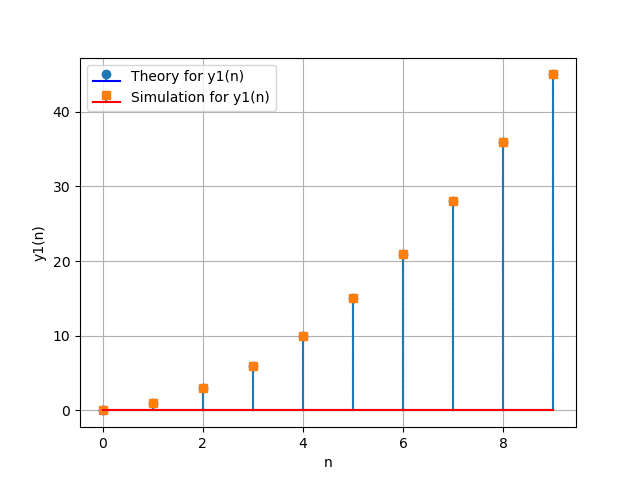
\includegraphics[width=0.5\textwidth]{ncert-maths/12/9/5/24/figs/y_1(n).png}
    \caption{Simulation vs Theory for y1(n)}
    \label{fig:12.9.5-24-1}
\end{figure}  

\begin{figure}[htbp]
    \centering
    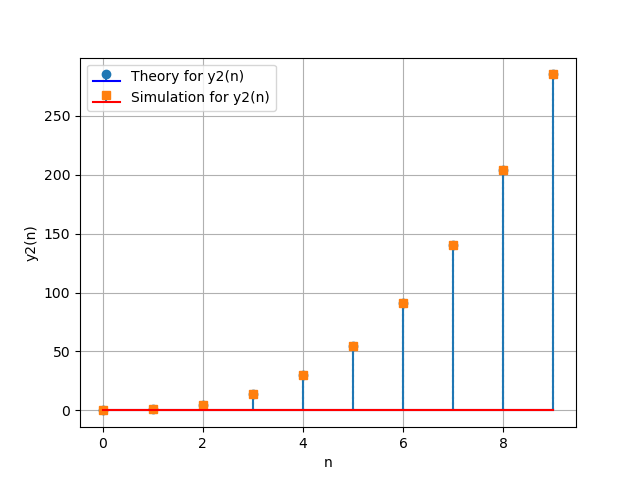
\includegraphics[width=0.5\textwidth]{ncert-maths/12/9/5/24/figs/y_2(n).png}
    \caption{Simulation vs Theory for y2(n)}
    \label{fig:12.9.5-24-2}
\end{figure}   

\begin{figure}[htbp]
    \centering
    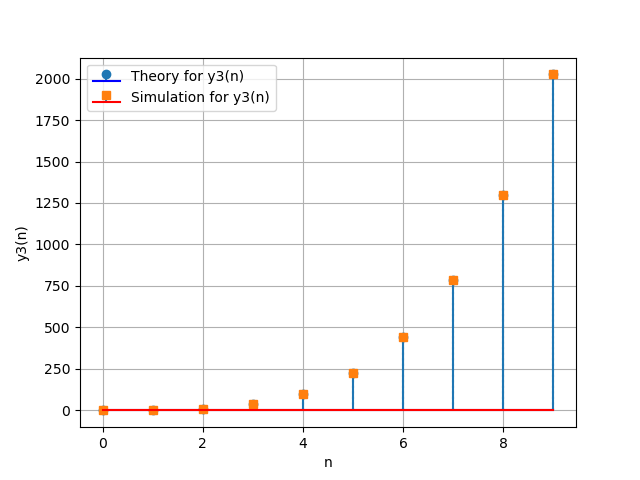
\includegraphics[width=0.5\textwidth]{ncert-maths/12/9/5/24/figs/y_3(n).png}
    \caption{Simulation vs Theory for y3(n) }
    \label{fig:12.9.5-24-3}
\end{figure} 
%\end{document}
